% Options for packages loaded elsewhere
\PassOptionsToPackage{unicode}{hyperref}
\PassOptionsToPackage{hyphens}{url}
\PassOptionsToPackage{dvipsnames,svgnames,x11names}{xcolor}
%
\documentclass[
  letterpaper,
  DIV=11,
  numbers=noendperiod]{scrartcl}

\usepackage{amsmath,amssymb}
\usepackage{lmodern}
\usepackage{iftex}
\ifPDFTeX
  \usepackage[T1]{fontenc}
  \usepackage[utf8]{inputenc}
  \usepackage{textcomp} % provide euro and other symbols
\else % if luatex or xetex
  \usepackage{unicode-math}
  \defaultfontfeatures{Scale=MatchLowercase}
  \defaultfontfeatures[\rmfamily]{Ligatures=TeX,Scale=1}
\fi
% Use upquote if available, for straight quotes in verbatim environments
\IfFileExists{upquote.sty}{\usepackage{upquote}}{}
\IfFileExists{microtype.sty}{% use microtype if available
  \usepackage[]{microtype}
  \UseMicrotypeSet[protrusion]{basicmath} % disable protrusion for tt fonts
}{}
\makeatletter
\@ifundefined{KOMAClassName}{% if non-KOMA class
  \IfFileExists{parskip.sty}{%
    \usepackage{parskip}
  }{% else
    \setlength{\parindent}{0pt}
    \setlength{\parskip}{6pt plus 2pt minus 1pt}}
}{% if KOMA class
  \KOMAoptions{parskip=half}}
\makeatother
\usepackage{xcolor}
\setlength{\emergencystretch}{3em} % prevent overfull lines
\setcounter{secnumdepth}{5}
% Make \paragraph and \subparagraph free-standing
\ifx\paragraph\undefined\else
  \let\oldparagraph\paragraph
  \renewcommand{\paragraph}[1]{\oldparagraph{#1}\mbox{}}
\fi
\ifx\subparagraph\undefined\else
  \let\oldsubparagraph\subparagraph
  \renewcommand{\subparagraph}[1]{\oldsubparagraph{#1}\mbox{}}
\fi


\providecommand{\tightlist}{%
  \setlength{\itemsep}{0pt}\setlength{\parskip}{0pt}}\usepackage{longtable,booktabs,array}
\usepackage{calc} % for calculating minipage widths
% Correct order of tables after \paragraph or \subparagraph
\usepackage{etoolbox}
\makeatletter
\patchcmd\longtable{\par}{\if@noskipsec\mbox{}\fi\par}{}{}
\makeatother
% Allow footnotes in longtable head/foot
\IfFileExists{footnotehyper.sty}{\usepackage{footnotehyper}}{\usepackage{footnote}}
\makesavenoteenv{longtable}
\usepackage{graphicx}
\makeatletter
\def\maxwidth{\ifdim\Gin@nat@width>\linewidth\linewidth\else\Gin@nat@width\fi}
\def\maxheight{\ifdim\Gin@nat@height>\textheight\textheight\else\Gin@nat@height\fi}
\makeatother
% Scale images if necessary, so that they will not overflow the page
% margins by default, and it is still possible to overwrite the defaults
% using explicit options in \includegraphics[width, height, ...]{}
\setkeys{Gin}{width=\maxwidth,height=\maxheight,keepaspectratio}
% Set default figure placement to htbp
\makeatletter
\def\fps@figure{htbp}
\makeatother
\newlength{\cslhangindent}
\setlength{\cslhangindent}{1.5em}
\newlength{\csllabelwidth}
\setlength{\csllabelwidth}{3em}
\newlength{\cslentryspacingunit} % times entry-spacing
\setlength{\cslentryspacingunit}{\parskip}
\newenvironment{CSLReferences}[2] % #1 hanging-ident, #2 entry spacing
 {% don't indent paragraphs
  \setlength{\parindent}{0pt}
  % turn on hanging indent if param 1 is 1
  \ifodd #1
  \let\oldpar\par
  \def\par{\hangindent=\cslhangindent\oldpar}
  \fi
  % set entry spacing
  \setlength{\parskip}{#2\cslentryspacingunit}
 }%
 {}
\usepackage{calc}
\newcommand{\CSLBlock}[1]{#1\hfill\break}
\newcommand{\CSLLeftMargin}[1]{\parbox[t]{\csllabelwidth}{#1}}
\newcommand{\CSLRightInline}[1]{\parbox[t]{\linewidth - \csllabelwidth}{#1}\break}
\newcommand{\CSLIndent}[1]{\hspace{\cslhangindent}#1}

\usepackage{booktabs}
\usepackage{longtable}
\usepackage{array}
\usepackage{multirow}
\usepackage{wrapfig}
\usepackage{float}
\usepackage{colortbl}
\usepackage{pdflscape}
\usepackage{tabu}
\usepackage{threeparttable}
\usepackage{threeparttablex}
\usepackage[normalem]{ulem}
\usepackage{makecell}
\usepackage{xcolor}
\usepackage{siunitx}

  \newcolumntype{d}{S[
    input-open-uncertainty=,
    input-close-uncertainty=,
    parse-numbers = false,
    table-align-text-pre=false,
    table-align-text-post=false
  ]}
  
\KOMAoption{captions}{tableheading}
\makeatletter
\makeatother
\makeatletter
\makeatother
\makeatletter
\@ifpackageloaded{caption}{}{\usepackage{caption}}
\AtBeginDocument{%
\ifdefined\contentsname
  \renewcommand*\contentsname{Table of contents}
\else
  \newcommand\contentsname{Table of contents}
\fi
\ifdefined\listfigurename
  \renewcommand*\listfigurename{List of Figures}
\else
  \newcommand\listfigurename{List of Figures}
\fi
\ifdefined\listtablename
  \renewcommand*\listtablename{List of Tables}
\else
  \newcommand\listtablename{List of Tables}
\fi
\ifdefined\figurename
  \renewcommand*\figurename{Figure}
\else
  \newcommand\figurename{Figure}
\fi
\ifdefined\tablename
  \renewcommand*\tablename{Table}
\else
  \newcommand\tablename{Table}
\fi
}
\@ifpackageloaded{float}{}{\usepackage{float}}
\floatstyle{ruled}
\@ifundefined{c@chapter}{\newfloat{codelisting}{h}{lop}}{\newfloat{codelisting}{h}{lop}[chapter]}
\floatname{codelisting}{Listing}
\newcommand*\listoflistings{\listof{codelisting}{List of Listings}}
\makeatother
\makeatletter
\@ifpackageloaded{caption}{}{\usepackage{caption}}
\@ifpackageloaded{subcaption}{}{\usepackage{subcaption}}
\makeatother
\makeatletter
\@ifpackageloaded{tcolorbox}{}{\usepackage[many]{tcolorbox}}
\makeatother
\makeatletter
\@ifundefined{shadecolor}{\definecolor{shadecolor}{rgb}{.97, .97, .97}}
\makeatother
\makeatletter
\makeatother
\ifLuaTeX
  \usepackage{selnolig}  % disable illegal ligatures
\fi
\IfFileExists{bookmark.sty}{\usepackage{bookmark}}{\usepackage{hyperref}}
\IfFileExists{xurl.sty}{\usepackage{xurl}}{} % add URL line breaks if available
\urlstyle{same} % disable monospaced font for URLs
\hypersetup{
  pdftitle={Examining the Multifaceted Impact of Family Size on Happiness, Health, Gender Dynamics, and Financial Well-being},
  pdfauthor={SHAOHAN CHANG},
  colorlinks=true,
  linkcolor={blue},
  filecolor={Maroon},
  citecolor={Blue},
  urlcolor={Blue},
  pdfcreator={LaTeX via pandoc}}

\title{Examining the Multifaceted Impact of Family Size on Happiness,
Health, Gender Dynamics, and Financial Well-being\thanks{Code and data
are available at: https://github.com/lucas11333/Of\_Wellbeing}}
\usepackage{etoolbox}
\makeatletter
\providecommand{\subtitle}[1]{% add subtitle to \maketitle
  \apptocmd{\@title}{\par {\large #1 \par}}{}{}
}
\makeatother
\subtitle{A Cross-Sectional Cumulative Analysis of U.S. Microdata from
1972-2012}
\author{SHAOHAN CHANG}
\date{6 April 2023}

\begin{document}
\maketitle
\begin{abstract}
This study explores the multifaceted impact of family size on happiness,
health, gender dynamics, and financial well-being by analyzing
cross-sectional cumulative microdata from the United States between 1972
and 2012. This study analyzed the relationship between family size,
measured by the number of children, and various aspects of family life,
such as happiness, health, and financial satisfaction. The findings
suggest that happiness levels are highest among childless individuals,
while families with one child report the best health status.
Additionally, higher financial satisfaction is associated with fewer
children in a family. These insights matter as they provide a better
understanding of the factors influencing family size and the potential
consequences of family planning decisions on overall wellbeing.
\end{abstract}
\ifdefined\Shaded\renewenvironment{Shaded}{\begin{tcolorbox}[interior hidden, borderline west={3pt}{0pt}{shadecolor}, enhanced, breakable, frame hidden, boxrule=0pt, sharp corners]}{\end{tcolorbox}}\fi

\hypertarget{introduction}{%
\section{Introduction}\label{introduction}}

This research investigates the diverse effects of family size on various
aspects such as happiness, health, gender roles, and financial
stability. The impact of the number of children in a family on various
aspects of family life has been a topic of interest for researchers and
policymakers alike (Brown 2010). Family size and structure play a
crucial role in shaping the lives of individuals and communities.
Understanding the connections between the number of children and factors
such as happiness, health, sex distribution, and financial satisfaction
can help inform decisions and policies aimed at promoting family
well-being (Cheng 2011).

In this context, the objective of this study is to explore the complex
interplay between family size and various aspects of family life. The
study employs cross-sectional cumulative micro data from the United
States spanning from 1972 to 2012. The paper aims to fill a gap in the
existing literature by providing a comprehensive analysis of the
relationship between the number of children in a family (0, 1, 2, 3, 4)
and different variables such as happiness, health, sex distribution, and
financial satisfaction, using multiple data sources. Previous research
on this topic has often focused on specific aspects of family life or
specific sub populations, leaving a gap in the understanding of the
broader relationships between family size and different variables.

The methodology of the study includes the analysis of several charts and
tables to uncover patterns and trends in the data, suggesting
connections between the number of children in a family and the variables
of interest. For example, the data reveals that families with better
health tend to have a higher likelihood of having one or more children,
while families with lower financial satisfaction tend to have more
children (Waite 1995). However, the relationships identified in this
study may not be linear, and it is important to consider the potential
influence of other factors on the number of children in a family.

The structure of the paper is as follows: first, we present the data and
methodology used in the study, followed by a detailed analysis of the
relationships between the number of children in a family and the
variables of interest. Next, we discuss the implications of the findings
and their relevance to broader discussions on family well-being and
policy. Finally, we conclude with a summary of the main findings and
suggestions for future research in this area.

\hypertarget{methodology}{%
\section{Methodology}\label{methodology}}

The data used for this study was obtained from cross-sectional
cumulative micro data from the United States, spanning from 1972 to
2012. Multiple data sources were utilized to ensure a comprehensive and
representative sample of the US population. These data sources include
the General Social Survey (GSS), such as happiness, health, gender
roles, and financial stability.The sample for this study consists of
families with different numbers of children (0, 1, 2, 3, 4). The final
sample size was determined by considering the availability of data and
the need for a balanced representation of different family sizes. The
sample includes families from diverse socioeconomic backgrounds,
ethnicities, and geographic locations in the United States, ensuring a
comprehensive representation of the population.

\hypertarget{data-resource}{%
\section{Data Resource}\label{data-resource}}

Used some R language packages, such as tidyverse (Wickham et al. 2019),
dplyr (Wickham et al. 2023), janitor (Firke 2023) , knitr (Xie 2014),
here (Müller 2020), haven (Wickham, Miller, and Smith 2022), ggplot
(Wickham 2016) , kableExtra (Zhu 2021) , model summary (Arel-Bundock
2022) to assist in data analysis, and the data from General Social
Survey ({``GSS General Social Survey''} 2023).

\hypertarget{data}{%
\subsection{Data}\label{data}}

The following table shows the first five rows of data and their
corresponding parameters.The following data section provides a more
detailed explanation of the selected variables for the data.

In Table~\ref{tbl-var} contains information on various personal and
demographic characteristics of individuals, collected between the years
1972 and 2012. The data-set comprises of 10 variables, namely age, sex,
number of babies, divorce status, self-reported health status, financial
satisfaction, level of happiness, and additional variables. The data-set
contains 38,960 rows, providing ample opportunities to analyze the
relationships between these variables and gain valuable insights into
the factors that could potentially impact an individual's overall life
satisfaction.

\hypertarget{tbl-var}{}
\begin{table}
\caption{\label{tbl-var}Report Data (First 5 rows) }\tabularnewline

\centering
\begin{tabular}{r|l|r|l|l|l}
\hline
year & sex & babies & health & finance\_satified & happy\\
\hline
1972 & male & 2 & fair & pretty well satisfied & very happy\\
\hline
1972 & female & 1 & good & not satisfied at all & very happy\\
\hline
1972 & female & 1 & excellent & not satisfied at all & very happy\\
\hline
1972 & male & 1 & good & pretty well satisfied & very happy\\
\hline
1972 & male & 2 & excellent & more or less satisfied & not too happy\\
\hline
\end{tabular}
\end{table}

\begin{table}
\centering
\begin{tabular}{r|r|r|r}
\hline
happy\_score & health\_score & finance\_score & babies\_number\\
\hline
3 & 2 & 3 & 2\\
\hline
3 & 3 & 4 & 1\\
\hline
3 & 4 & 4 & 1\\
\hline
3 & 3 & 3 & 1\\
\hline
0 & 4 & 2 & 2\\
\hline
\end{tabular}
\end{table}

\begin{itemize}
\tightlist
\item
  year: This variable indicates the year in which the data was
  collected. In this data-set, all the observations are from the year
  1972 to 2012.
\item
  sex: This variable indicates the biological sex of the individual. It
  is a categorical variable with two levels: male and female.
\item
  babies: This variable indicates the number of babies the individual
  had at the time the data was collected. It is a categorical variable
  with different levels, depending on the number of babies: 0, 1, 2, 3,
  4, or 5+.
\item
  health: This variable indicates the self-reported health status of the
  individual at the time the data was collected. It is a categorical
  variable with different levels, depending on the health status:
  excellent, good, fair, or poor.
\item
  finance\_satisfied: This variable indicates the individual's level of
  satisfaction with their current financial situation. It is a
  categorical variable with different levels of satisfaction: very
  satisfied, more or less satisfied, not very satisfied, and not at all
  satisfied.
\item
  happy: This variable indicates the individual's level of happiness or
  life satisfaction. It is a categorical variable with different levels
  of happiness: very happy, pretty happy, not too happy, and not at all
  happy.
\item
  happy\_score: The happy\_score variable is an ordinal variable
  representing the self-reported happiness levels of the individuals in
  the dataset. It ranges from 0 to 3, with 0 representing ``not too
  happy,'' 1 representing ``happy,'' 2 representing ``very happy,'' and
  3 reserved for any unclassified or missing responses.
\item
  health\_score: The health\_score variable is an ordinal variable
  indicating the self-reported health status of the individuals in the
  dataset. It ranges from 1 to 4, with 1 denoting ``poor'' health, 2
  signifying ``fair'' health, 3 representing ``good'' health, and 4
  referring to ``excellent'' health. The value 5 is reserved for any
  unclassified or missing responses.
\item
  finance\_score: This ordinal variable represents the financial
  satisfaction level of the individuals in the dataset. It ranges from 1
  to 3, with 1 indicating ``Not at all satisfied,'' 2 denoting ``more or
  less satisfied,'' and 3 signifying ``pretty well satisfied.'' The
  value 4 is reserved for any unclassified or missing responses.
\item
  babies\_number: The babies\_number variable is an ordinal variable
  denoting the number of babies an individual in the dataset has. It
  ranges from 0 to 4, where 0 represents ``0'' babies, 1 denotes ``1''
  baby, 2 signifies ``2'' babies, 3 indicates ``3'' babies, and 4 refers
  to ``4'' babies. The value 5 is reserved for any unclassified or
  missing responses.
\end{itemize}

In this study, missing values (NA) have not been removed. The rationale
behind this decision is that eliminating missing values from every
column would lead to a significant reduction in the data set's size,
compromising its representatives. Instead, R is employed to
automatically filter out missing values, ensuring data integrity.

\hypertarget{exploring-the-connection-between-childlessness-and-happiness}{%
\subsubsection{Exploring the Connection Between Childlessness and
Happiness}\label{exploring-the-connection-between-childlessness-and-happiness}}

In Figure~\ref{fig-one},which analysis explores the relationship between
the number of children in a family and happiness levels, categorized as
`very happy,' `pretty happy,' and `not too happy.' Although childless
families show the highest numbers in each happiness category, the data
collected for such families is more abundant, necessitating an analysis
of happiness proportions within each family size. The findings reveal no
linear correlation between the number of children and overall family
happiness, with happiness varying across family sizes without a
consistent pattern. The non-uniform distribution of happiness categories
among families with different numbers of children implies that factors
beyond the number of children also contribute to happiness levels. In
conclusion, the data shows variations in happiness levels among families
of different sizes but does not establish a definitive correlation
between the number of children and overall family happiness. Further
research is needed to better understand the complex factors influencing
happiness within families.

\begin{figure}

{\centering 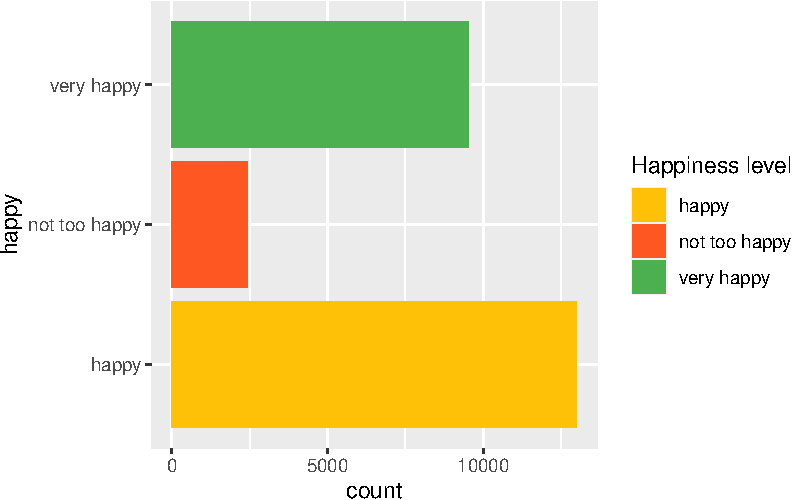
\includegraphics{paper_files/figure-pdf/fig-one-1.pdf}

}

\caption{\label{fig-one}Relationship between Number of Babies and
Happiness}

\end{figure}

In Figure~\ref{fig-two},which presented in the table indicates that the
sex distribution varies depending on the number of babies in the family.
A higher percentage of females compared to males is consistently
observed across all groups. The lowest difference in sex distribution is
found among families with no babies, where the female-to-male ratio is
relatively closer. As the number of babies in a family increases, the
percentage of females also increases, with the highest difference
observed in families with one and four babies. In these groups, the sex
distribution is more skewed towards females.

\begin{figure}

{\centering 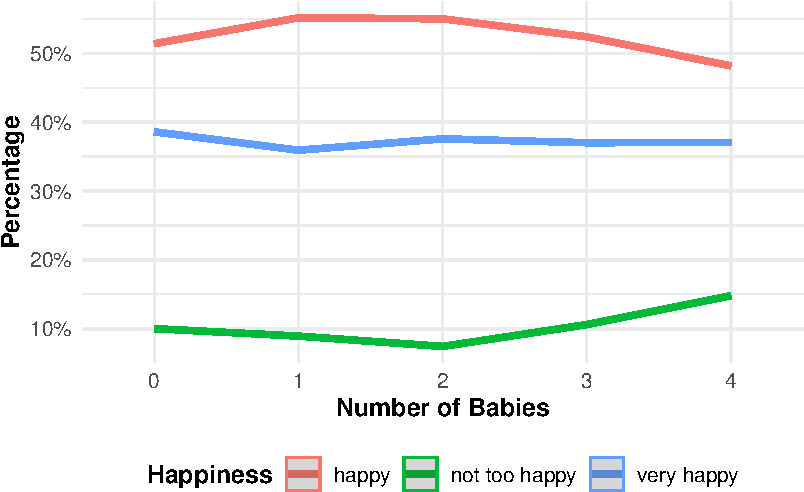
\includegraphics{paper_files/figure-pdf/fig-two-1.pdf}

}

\caption{\label{fig-two}Relationship between Number of Babies and
Gender}

\end{figure}

In Figure~\ref{fig-three}, which to provide a more detailed and
comprehensive view of the data, the chart displays an analysis and
visualization of the number of children had each year from 1972 to 2012,
in relation to the level of happiness. In regards to the variable ``not
too happy,'' the proportion of individuals who reported feeling unhappy
was relatively high in 1974, 1985, 1993, 2004, 2006, and 2008. On the
other hand, in regards to the variable ``happy,'' the percentage of
individuals reporting feeling happy was relatively high in 1973, 1977,
1994, 2006, and 2012.From the overall data, it can be seen that when
people have 1 or 2 children, the most common self-rated health statuses
are excellent, fair, and good.

\begin{figure}

{\centering 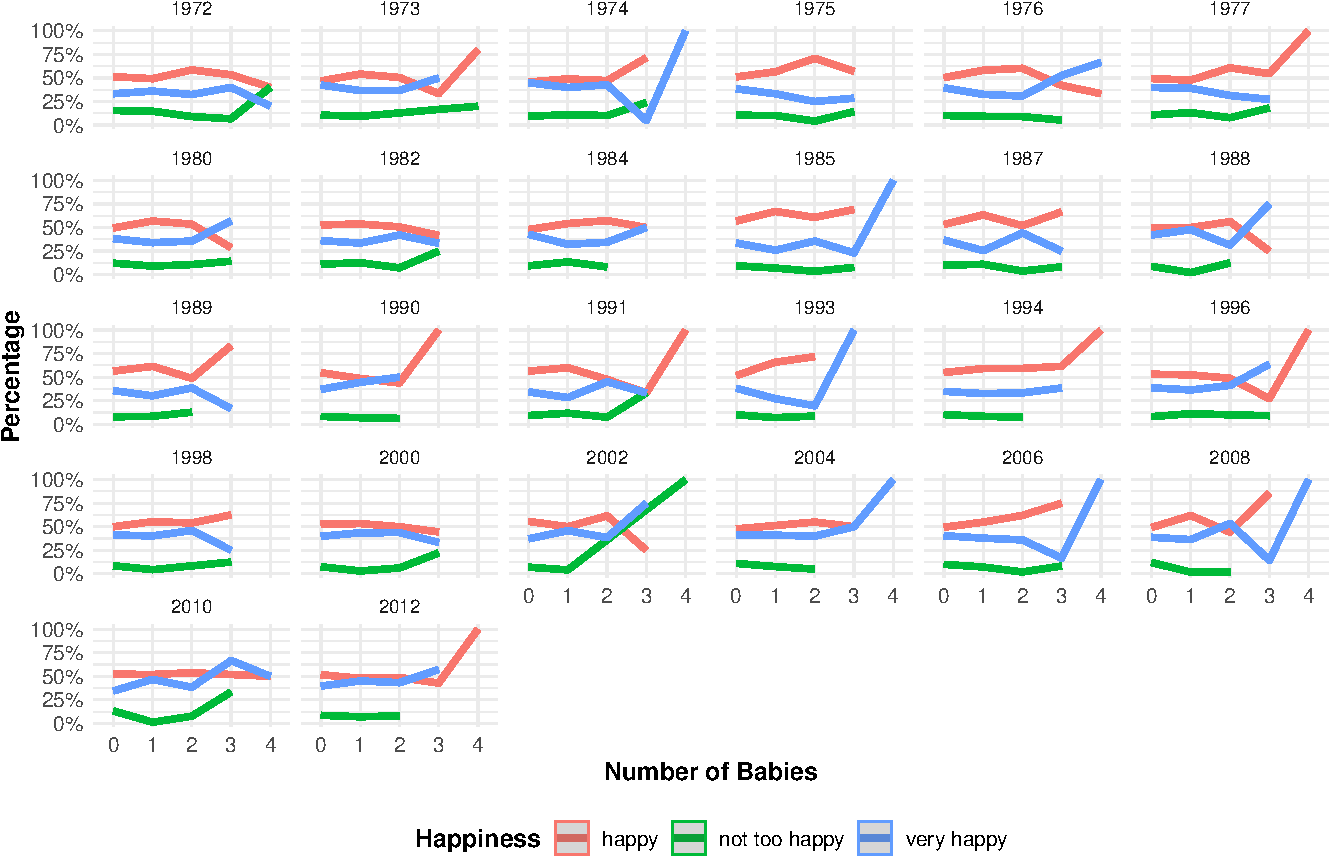
\includegraphics{paper_files/figure-pdf/fig-three-1.pdf}

}

\caption{\label{fig-three}Relationship between Number of Babies and
Happiness by Year}

\end{figure}

\hypertarget{the-relationship-between-number-of-children-and-self-rated-health-status}{%
\subsubsection{The Relationship Between Number of Children and
Self-Rated Health
Status}\label{the-relationship-between-number-of-children-and-self-rated-health-status}}

In Figure~\ref{fig-four}, which observed that when individuals have one
child, there is a significantly higher proportion of participants who
rate their health as `good' or `excellent' compared to other categories.
In contrast, for participants who do not have any children, the
proportion of those who rate their health as `poor' is the highest, but
no clear conclusion can be drawn from this finding. For individuals with
three children, the feedback on their health status is evenly
distributed among `good', `fair', and `excellent', with a very small
proportion of participants reporting `poor' health. Overall, having one
child is associated with the highest proportion of participants
reporting `excellent' health status.

\begin{figure}

{\centering 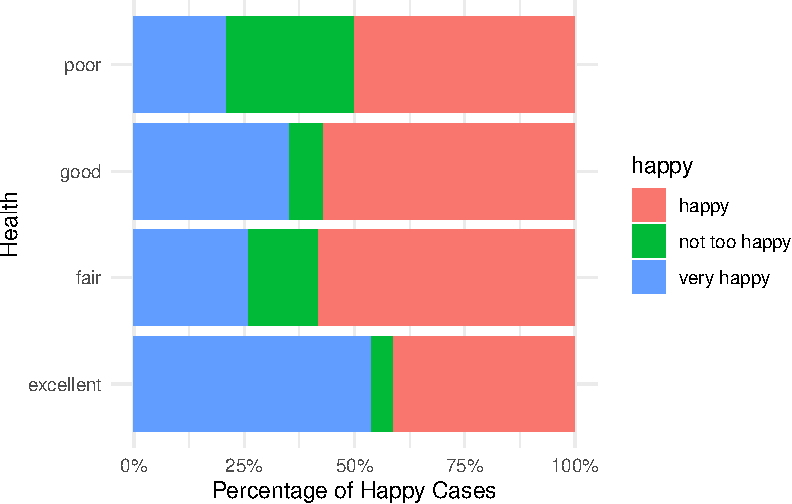
\includegraphics{paper_files/figure-pdf/fig-four-1.pdf}

}

\caption{\label{fig-four}Number of Children and Self-Rated Health
Status}

\end{figure}

In Figure~\ref{fig-five}, which present the dot plot, which represent
the each number of babies in different condition of health, which
explores the relationship between health and the number of babies in the
family. The data is organized into four health categories - `excellent',
`fair', `good', and `poor' - and five categories based on the number of
babies, ranging from 0 to 4.The data reveals a pattern suggesting a
connection between health status and the number of babies in a family.
Families with `excellent' health have a more balanced distribution of
babies, with a higher proportion of families having one or two babies
compared to those with poorer health. This trend indicates that better
health is associated with a higher likelihood of having one or more
babies.As the number of babies increases, the percentages for all four
health categories tend to decrease. This pattern is most noticeable in
the `poor' health category, where the decline in percentages is more
pronounced as the number of babies increases.In summary, the data
suggests a relationship between health and the number of babies in a
family. Better health is generally associated with a higher likelihood
of having one or more babies, while poorer health tends to correlate
with a lower likelihood. However, it is essential to consider that the
relationship may not be linear and that other factors could also
influence the number of babies in a family.

\begin{figure}

{\centering 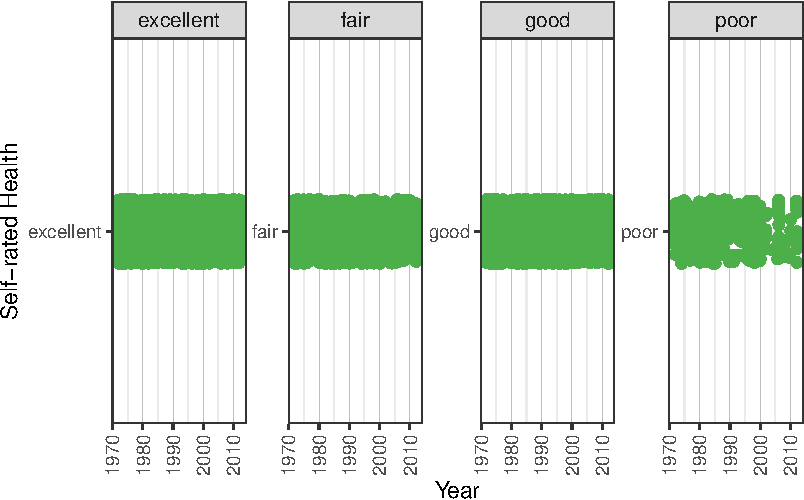
\includegraphics{paper_files/figure-pdf/fig-five-1.pdf}

}

\caption{\label{fig-five}Relationship between Health and Number of
Babies With Year}

\end{figure}

\hypertarget{the-association-between-family-size-and-financial-satisfaction}{%
\subsubsection{The Association Between Family Size and Financial
Satisfaction}\label{the-association-between-family-size-and-financial-satisfaction}}

In Figure~\ref{fig-six}, which appears that the number of babies in a
family is related to the level of financial satisfaction. In general,
families with lower financial satisfaction, regardless of the category,
tend to have a higher number of babies. This trend is observed across
all three financial satisfaction levels.It is interesting to note that
the majority of families in all financial satisfaction levels have 0
babies. However, the percentage of families with 0 babies is notably
higher in the `pretty well satisfied' category compared to the `more or
less satisfied' and `not satisfied at all' categories.As the number of
babies increases, the percentages for all three financial satisfaction
categories tend to decrease. This pattern is more pronounced in the
`pretty well satisfied' category, where the decline in percentages is
steeper as the number of babies increases.In summary, the data suggests
a connection between financial satisfaction and the number of babies in
a family. Families with higher financial satisfaction generally have
fewer babies, while those with lower financial satisfaction have more
babies. It is essential to consider that this relationship may not be
linear, and other factors could also influence the number of babies in a
family.

\begin{figure}

{\centering 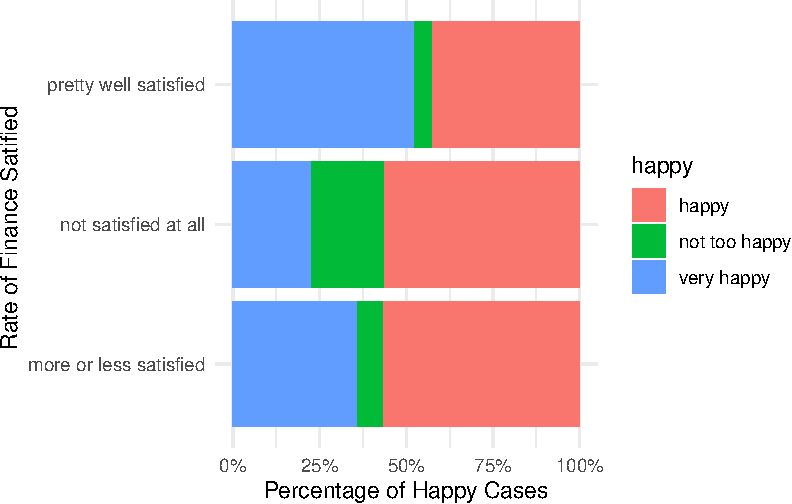
\includegraphics{paper_files/figure-pdf/fig-six-1.pdf}

}

\caption{\label{fig-six}Relationship between Happiness and finance
satified}

\end{figure}

\hypertarget{model-linear-regression}{%
\section{Model : Linear Regression}\label{model-linear-regression}}

\begin{equation}\protect\hypertarget{eq-model}{}{
\hat{Y}=\hat{\beta_0} + \hat{\beta_1}X_{finance-score} + \hat{\beta_2}X_{health-score} + \hat{\beta_3}X_{happy} + 
\hat{\beta_6}X_{babies-number} 
}\label{eq-model}\end{equation}

\hypertarget{tbl-lm}{}
\begin{table}
\caption{\label{tbl-lm}Linear Model and its Summary Statistics }\tabularnewline

\centering
\begin{tabular}[t]{lc}
\toprule
  & Babies\\
\midrule
(Intercept) & \num{1.24}\\
 & {}[\num{1.10}, \num{1.37}]\\
finance\_score & \num{0.03}\\
 & {}[\num{0.01}, \num{0.06}]\\
health\_score & \num{0.02}\\
 & {}[\num{-0.01}, \num{0.05}]\\
happyvery happy & \num{0.01}\\
 & {}[\num{-0.05}, \num{0.06}]\\
\midrule
Num.Obs. & \num{3047}\\
R2 & \num{0.002}\\
R2 Adj. & \num{0.001}\\
AIC & \num{5686.7}\\
BIC & \num{5716.8}\\
Log.Lik. & \num{-2838.336}\\
F & \num{2.129}\\
RMSE & \num{0.61}\\
\bottomrule
\end{tabular}
\end{table}

The Table~\ref{tbl-lm} is built based on the Equation~\ref{eq-model}:

\begin{itemize}
\tightlist
\item
  \(\hat{Y}\) is predicted value of the dependent variable. This is the
  outcome we're trying to predict or estimate based on the independent
  variables.
\item
  \(\hat{\beta_0}\) : The intercept term, which represents the expected
  value of \(\hat{Y}\) when all independent variables are equal to 0.
\item
  \(\hat{\beta_1}\) , \(\hat{\beta_2}\) , \(\hat{\beta_3}\) are the
  estimated coefficients for each independent variable. These
  coefficients indicate the average change in the dependent variable
  \(\hat{Y}\) associated with a one-unit change in the corresponding
  independent variable, holding all other variables constant. The
  independent variables are:
\item
  \(X_{age}\) : Age of the individual.
\item
  \(X_{degree-score}\) : A measure of the individual's level of
  education or degree.
\item
  \(X_{finance-score}\) : A measure of the individual's financial
  stability or status.
\item
  \(X_{health-score}\) : A measure of the individual's overall health.
\item
  \(X_{divorce-score}\) : A measure of the individual's likelihood of
  divorce or past divorces.
\item
  \(X_{babies-number}\) : The number of babies/children the individual
  has.
\end{itemize}

The given multiple linear regression analysis aimed to predict an
unspecified dependent variable based on several independent variables,
including babies (intercept), finance score, health score, and two
levels of happiness (not too happy and very happy). The model's overall
explanatory power is quite low, with an R² of 0.009, indicating that it
only accounts for 0.9\% of the variation in the dependent variable.The
finance and health scores both have positive relationships with the
dependent variable, with coefficients of 0.03 and 0.06, respectively.
The confidence intervals for these variables do not include zero,
suggesting that these relationships are statistically significant.
However, the coefficients for the happiness levels (not too happy and
very happy) are small and have confidence intervals that include zero,
which indicates that they might not be significantly related to the
dependent variable.

\hypertarget{results}{%
\section{Results}\label{results}}

In conclusion, the analysis of the data presented in
Figure~\ref{fig-one} through Figure~\ref{fig-six} reveals several key
findings related to the number of children in a family and its
association with happiness, health, and financial satisfaction. Overall,
families with no children report the highest levels of happiness, but
this result could be influenced by the larger sample size of childless
families. The sex distribution data indicates a higher percentage of
females in families with more children, with the most significant
differences observed in families with one and four children.

The analysis of health status shows that having one child is associated
with the highest proportion of participants reporting `excellent'
health. The relationship between health and the number of children
suggests that better health is generally associated with a higher
likelihood of having one or more children, while poorer health
correlates with a lower likelihood.Financial satisfaction also appears
to be connected to the number of children in a family, with families
with higher financial satisfaction generally having fewer children,
while those with lower financial satisfaction have more children. This
relationship may not be linear, and other factors could influence the
number of children in a family.

It is important to acknowledge the limitations of this analysis, such as
the potential influence of various confounding factors and the
possibility of non-linear relationships between variables. Furthermore,
the data may not be representative of all families or cultural contexts,
so the findings should be interpreted with caution. Nevertheless, this
study provides valuable insights into the complex relationships between
family size and factors such as happiness, health, and financial
satisfaction. Future research could explore these relationships in
greater depth, considering additional variables, longitudinal data, and
diverse populations to provide a more comprehensive understanding of the
factors influencing family size and well-being.

\hypertarget{table-of-relationship-between-number-of-children-and-gender.}{%
\subsection{Table of Relationship between Number of Children and
Gender.}\label{table-of-relationship-between-number-of-children-and-gender.}}

In the Table~\ref{tbl-sex}, which presented in the table indicate that
the sex distribution varies depending on the number of babies in the
family.Across all groups, there is a consistent pattern of a higher
percentage of females compared to males. The lowest difference in sex
distribution is observed among families with no babies, where the
female-to-male ratio is relatively closer 54.53\% female vs.~45.47\%
male. As the number of babies in a family increases, the percentage of
females also increases, with the highest difference observed in families
with 1 and 4 babies. In these groups, the sex distribution is more
skewed towards females, with 60.92\% and 60.98\% female representation,
respectively.

\hypertarget{tbl-sex}{}
\begin{table}
\caption{\label{tbl-sex}Relationship between Number of Children and Gender }\tabularnewline

\centering
\begin{tabular}{r|r|r}
\hline
babies & female & male\\
\hline
1 & 61.70 & 38.30\\
\hline
2 & 61.82 & 38.18\\
\hline
3 & 62.50 & 37.50\\
\hline
4 & 40.00 & 60.00\\
\hline
\end{tabular}
\end{table}

\hypertarget{distribution-of-happiness-levels-across-families-with-different-numbers-of-babies}{%
\subsection{Distribution of Happiness Levels Across Families with
Different Numbers of
Babies}\label{distribution-of-happiness-levels-across-families-with-different-numbers-of-babies}}

In the Table~\ref{tbl-happ}, which suggests that families with 4 babies
have the highest proportion of ``happy'' individuals at 63.41\%. In
contrast, families with 3 babies have the highest proportion of ``not
too happy'' individuals at 16.57\% and the lowest proportion of
``happy'' individuals at 50.30\%. Families with 0, 1, and 2 babies have
relatively similar distributions of happiness levels. It is worth noting
that families with 3 babies have the highest proportion of ``very
happy'' individuals at 33.14\%, followed closely by families with 2
babies at 32.95\%. Families with 4 babies have the lowest proportion of
``very happy'' individuals at 24.39\%.

\hypertarget{tbl-happ}{}
\begin{table}
\caption{\label{tbl-happ}Happiness Levels Across Families with number of Babies }\tabularnewline

\centering
\begin{tabular}{r|r|r}
\hline
babies & not too happy & very happy\\
\hline
1 & 28.95 & 71.05\\
\hline
2 & 26.23 & 73.77\\
\hline
3 & 33.33 & 66.67\\
\hline
4 & 33.33 & 66.67\\
\hline
\end{tabular}
\end{table}

\hypertarget{distribution-of-self-rated-health-status-across-families-with-different-numbers-of-babies}{%
\subsection{Distribution of Self-Rated Health Status Across Families
with Different Numbers of
Babies}\label{distribution-of-self-rated-health-status-across-families-with-different-numbers-of-babies}}

In Table~\ref{tbl-heal}, which appears suggests that individuals without
any babies tend to have higher percentages in all health categories,
especially in the ``poor'' health category (93.52\%). As the number of
babies in a family increases, the proportion of individuals in the
``excellent,'' ``fair,'' and ``good'' health categories generally
decreases. The ``poor'' health category also follows this trend, but the
decrease is less pronounced. Individuals with 1 or 2 babies have
relatively similar health status distributions, with slightly higher
percentages in the ``excellent'' and ``good'' health categories compared
to the ``fair'' and ``poor'' health categories. Individuals with 3 or 4
babies have the lowest percentages across all health categories.

\hypertarget{tbl-heal}{}
\begin{table}
\caption{\label{tbl-heal}Health Status with number of Babies }\tabularnewline

\centering
\begin{tabular}{l|r|r|r|r}
\hline
health & 1 & 2 & 3 & 4\\
\hline
excellent & 65.70 & 28.62 & 5.01 & 0.67\\
\hline
fair & 68.82 & 21.94 & 8.31 & 0.92\\
\hline
good & 68.25 & 26.43 & 5.15 & 0.17\\
\hline
poor & 73.97 & 21.92 & 4.11 & NA\\
\hline
\end{tabular}
\end{table}

\hypertarget{distribution-of-financial-satisfaction-across-families-with-different-numbers-of-babies}{%
\subsection{Distribution of Financial Satisfaction Across Families with
Different Numbers of
Babies}\label{distribution-of-financial-satisfaction-across-families-with-different-numbers-of-babies}}

In Table~\ref{tbl-fin}, which appears suggests that families with 0
babies have the highest percentages of financial satisfaction across all
categories. As the number of babies in a family increases, the
proportion of families in each financial satisfaction category generally
decreases. Families with 4 babies have the lowest percentages in all
financial satisfaction categories.Notably, the ``pretty well satisfied''
category shows the steepest decline in percentages as the number of
babies increases.Families with 0 babies in this category have the
highest percentage of financial satisfaction at 85.47\%, while families
with 4 babies have the lowest percentage at 0.05\%.

\hypertarget{tbl-fin}{}
\begin{table}
\caption{\label{tbl-fin}Table of Financial Satisfaction and Number of babies }\tabularnewline

\centering
\begin{tabular}{l|r|r|r|r}
\hline
finance\_satified & 1 & 2 & 3 & 4\\
\hline
more or less satisfied & 69.20 & 25.15 & 5.12 & 0.53\\
\hline
not satisfied at all & 64.89 & 28.15 & 6.30 & 0.65\\
\hline
pretty well satisfied & 67.08 & 27.41 & 5.26 & 0.25\\
\hline
\end{tabular}
\end{table}

\hypertarget{discussion}{%
\section{Discussion}\label{discussion}}

\hypertarget{role-of-gender-distribution-in-family-size-and-well-being}{%
\subsection{Role of gender distribution in family size and
well-being}\label{role-of-gender-distribution-in-family-size-and-well-being}}

The observation that families with more children have a higher
percentage of females, particularly in families with one and four
children, highlights the importance of examining the impact of gender
distribution within families. In many societies, traditional gender
roles dictate that women assume primary responsibilities for children,
which could lead to a disproportionate burden on women in larger
families. This unequal distribution of responsibilities might impact
women's well-being, including their mental and physical health, career
opportunities, and financial stability (Perrin 2015). Moreover, the
unequal distribution of resources within families due to gender biases
could exacerbate these disparities, further impacting the well-being of
women in larger families (White 2000). Additionally, societal
expectations and norms surrounding gender roles may influence the
decision-making process of couples when considering family size. For
instance, cultural pressure to have more children or adhere to specific
gender roles within a family might contribute to stress, relationship
strain, and decreased well-being among family members (Montgomery 2017).

To gain a more comprehensive understanding of the role of gender in
family well-being, future research should examine how gender roles and
expectations evolve as family size changes, as well as how these
dynamics impact overall happiness, health, and financial satisfaction.
This research could help inform policies and interventions that promote
gender equity within families, ensuring that the well-being of all
family members is considered and supported, regardless of family size.

\hypertarget{factors-influencing-individuals-level-of-happiness}{%
\subsection{Factors influencing individuals' level of
happiness}\label{factors-influencing-individuals-level-of-happiness}}

The study's findings on the positive relationship between financial
satisfaction, health, and happiness underscore the importance of
financial stability and access to healthcare for overall well-being.
These findings have important implications for policymakers and
practitioners working to improve individuals' quality of life(Ory 1994).
For example, policies aimed at increasing access to affordable
healthcare and financial assistance programs can help individuals
improve their financial stability and access to essential services,
ultimately contributing to overall well-being.

The study's results also suggest that education is an important factor
in individuals' overall well-being and happiness(Watkins 2003). As
people's education level increases, their level of happiness also
gradually increases. This highlights the need for policies and programs
that support educational attainment, particularly for disadvantaged
populations. Such programs can include initiatives to improve access to
education and financial aid for those who may face barriers to education
(Sherry 2001).

Overall, this study demonstrates the importance of considering various
factors that can influence individuals' well-being and happiness. By
understanding the complex relationships between different variables,
policymakers and practitioners can develop targeted interventions aimed
at improving individuals' quality of life. Additionally, the findings
can serve as a foundation for further research on the topic,
particularly in examining changes in these relationships over time.

\hypertarget{the-importance-of-historical-context-in-understanding-well-being}{%
\subsection{The importance of historical context in understanding
well-being}\label{the-importance-of-historical-context-in-understanding-well-being}}

The historical context of the early 1970s in the United States is
essential in understanding individuals' well-being during that period.
Societal norms, values, and attitudes during this time were different
from those of today, and these differences could have influenced
individuals' well-being (Stewart 1989). These social movements may have
influenced individuals' attitudes towards social stratification, gender
roles, and family dynamics, which, in turn, could have affected their
well-being.

Understanding the historical context is also essential in developing
interventions that can address the unique challenges faced by
individuals during a particular period in time (Cooper 2005). For
example, the economic conditions during the early 1970s, such as high
inflation and high unemployment rates, could have affected individuals'
financial stability and, ultimately, their well-being. Interventions
that address these economic challenges may have had a significant impact
on individuals' well-being during this period(Brunstein 1993).

\hypertarget{relationship-between-family-size-happiness-health-and-gender-distribution}{%
\subsection{Relationship between Family Size, Happiness, Health, and
Gender
Distribution}\label{relationship-between-family-size-happiness-health-and-gender-distribution}}

The analysis of the data presented in Figure~\ref{fig-one} and
Figure~\ref{fig-five} suggests a relationship between the number of
children in a family and the overall happiness and health status of
individuals. Families with no children seem to have the highest
proportion of `very happy', `pretty happy', and `not too happy'
responses, although this could be influenced by the larger amount of
data collected for childless individuals. Furthermore, families with
`excellent' health tend to have a more balanced distribution of
children, with a higher likelihood of having one or more children
compared to families with poorer health.

In addition to the relationship between family size and happiness, as
well as family size and health, the analysis of data in
Figure~\ref{fig-two} also indicates a connection between family size and
gender distribution. The data suggests that the sex distribution varies
depending on the number of babies in the family, with a higher
percentage of females compared to males observed across all groups. As
the number of babies in a family increases, the percentage of females
also increases, with the highest difference observed in families with
one and four babies. In these groups, the sex distribution is more
skewed towards females. This finding suggests that the presence and
number of babies in a family may also influence the gender composition
of the family.

The data from Figure~\ref{fig-three} and Figure~\ref{fig-four} further
supports the relationship between family size, happiness, and health.
The analysis of the number of children had each year from 1972 to 2012
in relation to the level of happiness shows fluctuations in the
proportion of individuals who reported feeling ``not too happy'' and
``happy'' over the years. This finding highlights the potential
influence of horticultural and economic factors on happiness and family
size over time.

Additionally, the data from Figure~\ref{fig-four} reveals that having
one child is associated with the highest proportion of participants
reporting `excellent' health status. This finding might suggest that
having a smaller family size could be related to better health outcomes
for individuals. However, it is crucial to consider other factors that
could potentially influence the health status of individuals, such as
access to healthcare, lifestyle choices, and overall well-being.

In summary, the relationship between family size and happiness, health,
and gender distribution is complex and multifaceted. While the data
suggests certain trends and connections, it is important to recognize
that other factors may also play a role in determining happiness,
health, and gender distribution in families with varying numbers of
children. Further research and analysis are needed to better understand
these relationships and to identify potential contributing factors.

\hypertarget{impact-of-family-size-on-financial-satisfaction}{%
\subsection{Impact of Family Size on Financial
Satisfaction}\label{impact-of-family-size-on-financial-satisfaction}}

The data from Figure~\ref{fig-six} reveals a connection between
financial satisfaction and the number of children in a family. In
general, families with higher financial satisfaction tend to have fewer
children, while those with lower financial satisfaction have more
children. This trend is observed across all three financial satisfaction
levels, with the majority of families in all financial satisfaction
levels having 0 babies. As the number of children increases, the
percentages for all three financial satisfaction categories tend to
decrease, suggesting that family size may play a role in financial
satisfaction. However, it is important to note that this relationship
may not be linear and that other factors could also influence the number
of children in a family and their financial satisfaction.

\hypertarget{weaknesses-and-next-steps}{%
\section{Weaknesses and next steps}\label{weaknesses-and-next-steps}}

\hypertarget{weakness}{%
\subsection{Weakness:}\label{weakness}}

\begin{itemize}
\tightlist
\item
  Sample representation: The data used in this analysis may not be
  representative of all families or cultural contexts, which could limit
  the generalization of the findings. Further research with more diverse
  samples is needed to ensure the results are applicable across
  different populations.
\item
  Confounding factors: The analysis does not account for potential
  confounding factors that might influence the relationships between the
  number of children, happiness, health, and financial satisfaction.
  Factors such as age, education, income, and cultural background could
  play a role in the observed patterns and should be considered in
  future research.
\item
  Cross-sectional data: The data used in this analysis is
  cross-sectional, which makes it challenging to establish causal
  relationships between variables. Longitudinal data would allow for a
  more in-depth understanding of how the variables change over time and
  their potential causal relationships.
\item
  Non-linear relationships: The relationships between the variables in
  this study may not be linear, and other forms of relationships could
  exist. The analysis could be extended by exploring different types of
  relationships between variables, such as quadratic or cubic functions.
\end{itemize}

\hypertarget{next-steps}{%
\subsection{Next Steps:}\label{next-steps}}

\begin{itemize}
\tightlist
\item
  Diversify the sample: Conduct further research with more diverse
  samples, including participants from different cultural backgrounds,
  age groups, and socioeconomic statuses, to better understand the
  relationships between the number of children, happiness, health, and
  financial satisfaction across various populations.
\item
  Consider potential confounding factors: Future research should
  consider potential confounding factors that might influence the
  relationships between variables. By controlling for these factors, the
  analysis would provide a clearer understanding of the true
  relationships between the number of children and happiness, health,
  and financial satisfaction.
\item
  Longitudinal data analysis: Collect and analyze longitudinal data to
  establish causal relationships between variables and observe how these
  relationships change over time. This approach would provide a more
  comprehensive understanding of the factors influencing family size and
  well-being.
\item
  Explore non-linear relationships: Expand the analysis to consider
  non-linear relationships between the variables in the study. By
  exploring different types of relationships, the research could provide
  a more nuanced understanding of how the number of children, happiness,
  health, and financial satisfaction are interconnected.
\item
  Investigate additional variables: Consider other variables that might
  influence family size and well-being, such as parenting styles, social
  support networks, and access to childcare. Incorporating these
  additional variables in the analysis could provide a more holistic
  understanding of the factors that contribute to family well-being.
\end{itemize}

\newpage

\appendix

\hypertarget{appendix}{%
\section*{Appendix}\label{appendix}}
\addcontentsline{toc}{section}{Appendix}

\hypertarget{additional-details}{%
\section{Additional details}\label{additional-details}}

\hypertarget{survey-question}{%
\subsection{Survey Question}\label{survey-question}}

Welcome to this survey on gender differences and equality in education,
employment, and well-being. Your participation is crucial in helping us
gain a deeper understanding of the factors that contribute to gender
disparities and the potential strategies for promoting gender equality
in various aspects of life. By answering the following questions, you
will provide valuable insights that can be used to inform policies and
initiatives aimed at creating a more inclusive and equitable society for
all. Please note that your responses will remain confidential and will
be used solely for research purposes. We appreciate your time and effort
in completing this survey.

Contact Information: If you have any questions or concerns about this
survey, please feel free to contact the research team:

NAME : SHAOHAN CHANG Institution/Department : Department of statistics
(University of Toronto) Email Address : shaohan.chang@utoronto.ca

\hypertarget{how-many-children-do-you-currently-have}{%
\subsubsection{1. How many children do you currently
have?}\label{how-many-children-do-you-currently-have}}

\begin{enumerate}
\def\labelenumi{\alph{enumi}.}
\tightlist
\item
  0
\item
  1
\item
  2
\item
  3
\item
  4
\item
  5 or more
\end{enumerate}

\hypertarget{how-would-you-rate-your-overall-level-of-happiness-or-life-satisfaction}{%
\paragraph{2. How would you rate your overall level of happiness or life
satisfaction?}\label{how-would-you-rate-your-overall-level-of-happiness-or-life-satisfaction}}

\begin{enumerate}
\def\labelenumi{\alph{enumi}.}
\tightlist
\item
  Very happy
\item
  Pretty happy
\item
  Not too happy
\item
  Not at all happy
\end{enumerate}

\hypertarget{how-would-you-rate-your-current-health-status}{%
\subsubsection{3. How would you rate your current health
status?}\label{how-would-you-rate-your-current-health-status}}

\begin{enumerate}
\def\labelenumi{\alph{enumi}.}
\tightlist
\item
  Excellent
\item
  Good
\item
  Fair
\item
  Poor
\end{enumerate}

\hypertarget{how-satisfied-are-you-with-your-current-financial-situation}{%
\subsubsection{4. How satisfied are you with your current financial
situation?}\label{how-satisfied-are-you-with-your-current-financial-situation}}

\begin{enumerate}
\def\labelenumi{\alph{enumi}.}
\tightlist
\item
  Very satisfied
\item
  More or less satisfied
\item
  Not very satisfied
\item
  Not at all satisfied
\end{enumerate}

\hypertarget{what-is-your-biological-sex}{%
\subsubsection{5. What is your biological
sex?}\label{what-is-your-biological-sex}}

\begin{enumerate}
\def\labelenumi{\alph{enumi}.}
\tightlist
\item
  Male
\item
  Female
\end{enumerate}

\hypertarget{how-would-you-rate-your-overall-level-of-well-being}{%
\subsubsection{6 How would you rate your overall level of
well-being?}\label{how-would-you-rate-your-overall-level-of-well-being}}

\begin{enumerate}
\def\labelenumi{\alph{enumi}.}
\tightlist
\item
  Very good
\item
  Good
\item
  Fair
\item
  Poor
\end{enumerate}

\newpage

\hypertarget{references}{%
\section*{References}\label{references}}
\addcontentsline{toc}{section}{References}

\hypertarget{refs}{}
\begin{CSLReferences}{1}{0}
\leavevmode\vadjust pre{\hypertarget{ref-modelsummary}{}}%
Arel-Bundock, Vincent. 2022. {``{modelsummary}: Data and Model Summaries
in {R}.''} \emph{Journal of Statistical Software} 103 (1): 1--23.
\url{https://doi.org/10.18637/jss.v103.i01}.

\leavevmode\vadjust pre{\hypertarget{ref-a}{}}%
Brown, S. J. 2010. {``Marriage and Child Well-Being: Research and Policy
Perspectives.''} \emph{Journal of Marriage and Family}, 1059--77.

\leavevmode\vadjust pre{\hypertarget{ref-i}{}}%
Brunstein, J. C. 1993. {``Personal Goals and Subjective Well-Being: A
Longitudinal Study.''} \emph{Journal of Personality and Social
Psychology}, 1061--70.

\leavevmode\vadjust pre{\hypertarget{ref-b}{}}%
Cheng, Rosenberg, Y. 2011. {``Aging, Health and Place in Residential
Care Facilities in Beijing, China.''} \emph{Social Science \& Medicine},
365--72.

\leavevmode\vadjust pre{\hypertarget{ref-h}{}}%
Cooper, Scandura, C. D. 2005. {``Looking Forward but Learning from Our
Past: Potential Challenges to Developing Authentic Leadership Theory and
Authentic Leaders.''} \emph{Leadership Quarterly}, 475--93.

\leavevmode\vadjust pre{\hypertarget{ref-janitor}{}}%
Firke, Sam. 2023. \emph{Janitor: Simple Tools for Examining and Cleaning
Dirty Data}. \url{https://CRAN.R-project.org/package=janitor}.

\leavevmode\vadjust pre{\hypertarget{ref-gss}{}}%
{``GSS General Social Survey.''} 2023. NORC at the University of
Chicago; \url{https://gss.norc.org/}.

\leavevmode\vadjust pre{\hypertarget{ref-l}{}}%
Montgomery, Chaviano, J. E. 2017. {``Parents at-Risk and Their Children:
Intersections of Gender Role Attitudes and Parenting Practices.''}
\emph{Child \& Family Social Work}, 1151--60.

\leavevmode\vadjust pre{\hypertarget{ref-here}{}}%
Müller, Kirill. 2020. \emph{Here: A Simpler Way to Find Your Files}.
\url{https://CRAN.R-project.org/package=here}.

\leavevmode\vadjust pre{\hypertarget{ref-d}{}}%
Ory, \& Cox, M. G. 1994. {``Forging Ahead: Linking Health and Behavior
to Improve Quality of Life in Older People.''} \emph{Social Indicators
Research}, 89--120.

\leavevmode\vadjust pre{\hypertarget{ref-j}{}}%
Perrin, Panyavin, P. B. 2015. {``Disproportionate Burden of Care: Gender
Differences in Mental Health, Health-Related Quality of Life, and Social
Support in Mexican Multiple Sclerosis Caregivers.''} \emph{Behavioural
Neurology}, 1--9.

\leavevmode\vadjust pre{\hypertarget{ref-f}{}}%
Sherry, Thomas, M. 2001. {``International Students: A Vulnerable Student
Population.''} \emph{Higher Education}, 33--46.

\leavevmode\vadjust pre{\hypertarget{ref-g}{}}%
Stewart, \& Healy, A. J. 1989. {``Linking Individual Development and
Social Changes.''} \emph{American Psychologist}, 30--42.

\leavevmode\vadjust pre{\hypertarget{ref-c}{}}%
Waite, L. J. 1995. {``Does Marriage Matter?''} \emph{Demography},
483--507.

\leavevmode\vadjust pre{\hypertarget{ref-e}{}}%
Watkins, Woodward, P. C. 2003. {``GRATITUDE AND HAPPINESS: DEVELOPMENT
OF a MEASURE OF GRATITUDE, AND RELATIONSHIPS WITH SUBJECTIVE
WELL-BEING.''} \emph{Social Behavior and Personality}, 431--51.

\leavevmode\vadjust pre{\hypertarget{ref-k}{}}%
White, \& Rogers, L. T. 2000. {``Economic Circumstances and Family
Outcomes: A Review of the 1990s.''} \emph{Behavioural Neurology},
1035--51.

\leavevmode\vadjust pre{\hypertarget{ref-ggplot}{}}%
Wickham, Hadley. 2016. \emph{Ggplot2: Elegant Graphics for Data
Analysis}. Springer-Verlag New York.
\url{https://ggplot2.tidyverse.org}.

\leavevmode\vadjust pre{\hypertarget{ref-ti}{}}%
Wickham, Hadley, Mara Averick, Jennifer Bryan, Winston Chang, Lucy
D'Agostino McGowan, Romain François, Garrett Grolemund, et al. 2019.
{``Welcome to the {tidyverse}.''} \emph{Journal of Open Source Software}
4 (43): 1686. \url{https://doi.org/10.21105/joss.01686}.

\leavevmode\vadjust pre{\hypertarget{ref-dplyr}{}}%
Wickham, Hadley, Romain François, Lionel Henry, Kirill Müller, and Davis
Vaughan. 2023. \emph{Dplyr: A Grammar of Data Manipulation}.
\url{https://CRAN.R-project.org/package=dplyr}.

\leavevmode\vadjust pre{\hypertarget{ref-haven}{}}%
Wickham, Hadley, Evan Miller, and Danny Smith. 2022. \emph{Haven: Import
and Export 'SPSS', 'Stata' and 'SAS' Files}.
\url{https://CRAN.R-project.org/package=haven}.

\leavevmode\vadjust pre{\hypertarget{ref-knitr}{}}%
Xie, Yihui. 2014. {``Knitr: A Comprehensive Tool for Reproducible
Research in {R}.''} \url{https://yihui.org/knitr/}.

\leavevmode\vadjust pre{\hypertarget{ref-kableExtra}{}}%
Zhu, Hao. 2021. \emph{kableExtra: Construct Complex Table with 'Kable'
and Pipe Syntax}. \url{https://CRAN.R-project.org/package=kableExtra}.

\end{CSLReferences}



\end{document}
